\def\year{2017}\relax
%File: formatting-instruction.tex
\documentclass[letterpaper]{article}
\usepackage{aaai17}
\usepackage{amsmath}
\usepackage{amsthm}
\usepackage{times}
\usepackage{helvet}
\usepackage{courier}
\usepackage{graphicx}
\usepackage{subfigure}
\usepackage{mdwmath}
\usepackage{mdwtab}
\usepackage{amssymb}
\usepackage{booktabs}
\usepackage{algorithm}
\usepackage{pifont}
\usepackage[noend]{algpseudocode}
\usepackage{balance}
\usepackage{bm}
\usepackage{ulem}
\usepackage{array}
\usepackage{balance}
\usepackage{multirow}
\usepackage{multicol}
\usepackage{threeparttable}
\frenchspacing
\setlength{\pdfpagewidth}{8.5in}
\setlength{\pdfpageheight}{11in}
\usepackage[marginal]{footmisc}
\usepackage{extarrows}
\usepackage{natbib}

\setcounter{secnumdepth}{0}  
 \begin{document}
% The file aaai.sty is the style file for AAAI Press 
% proceedings, working notes, and technical reports.
%
\title{Analysis of the Variance Reduction in SVRG and a New Acceleration Method}
%\author{
%}
\maketitle
\begin{abstract}
Stochastic gradient descent (SGD) with variance reduction  technique such as SVRG is efficient to train parameters of many machine learning models. Although many variants of SVRG have been proposed,  the analysis of variance has not been thoroughly discussed. Besides,  the variants of SVRG have to keep a snapshot of the full gradient in every epoch, which is computationally expensive. In this paper, we propose a framework EUI which is an abstraction of  the existing variants of SVRG, and then  provide a general and deep analysis of the variance from a new perspective. Moreover,   a new variant of SGD with the variance reduction technique named \textsc{sampleVR} is proposed. \textsc{sampleVR} replaces the full gradient computation with an estimation, thus decreasing gradient complexity significantly.  Both the theoretical analysis and the empirical studies show that \textsc{sampleVR} makes  training loss converge faster than its counterparts significantly. 
\end{abstract}

\section{Introduction}
\label{sect_introduction}
Many machine learning tasks such as classification and regression  can be  presented as solving the optimisation problem described as 
\begin{equation}
\label{equa_loss_minimization}
\min F(\omega),~~~~~F(\omega)=\frac{1}{n}\sum\limits_{i=1}^n f_i(\omega)+R(\omega).
\end{equation} where $F(\omega)$ denotes the training loss or the loss function. The training loss is the sum of a finite number of functions, i.e. $\nabla f_i(\omega)$ with $i\in\{1,2, ..., n\}$. $\omega$ is the parameter of the machine learning model, and $n$ represents the size of the training data. $R(\omega)$ is the regulariser  which is used to prevent overfitting.    



Gradient descent (GD) is used to train the parameters for such underlying machine learning tasks. Since GD computes a full gradient every iteration for training parameters, it has to perform a large amount of gradient calculations.  This would affect the performance significantly in the presence of a large amount of training data. The stochastic gradient descent (SGD) improves time efficiency by using stochastic gradients instead of the full gradient to train parameters. However, variance caused by the stochastic gradients usually impairs convergence of the training loss. Specifically, when the parameters are close to the optimum, it is increasingly difficult to make a further progress  due to the variance. Conventional studies show that a decaying learning rate can be used to decrease the variance. But the training loss converges slowly when the learning rate is small. 

Recently, \citet{Johnson:9MAvkbgy} improve SGD with the variance reduction technique named SVRG which uses a constant learning rate to train the parameters.  Based on the variance reduction technique adopted by SVRG, many variants of SVRG such as S2GD \citep{Richtarik:2013te}, mS2GD \citep{Liu:2015bx}, EMGD \citep{Zhang2013Linear}, SVR-GHT \citep{Li:2016vh}, Prox-SVRG \citep{Xiao:2014vw}, SVRG++ \citep{Allen2015Improved}, and Katyusha \citep{Allenzhu2016Katyusha} have been proposed. However, the analysis of the variance, which is essential to understand and exploit the variance reduction technique, lacks enough discussion. \citet{AllenZhu:2016up} have  presented some impressive analysis of the variance. However, such technical analysis is obtained under the specific settings of an algorithm, which lacks the generality. Although the analysis provides an upper bound of the variance, it lacks the result of the lower bound. Besides, those existing algorithms are organised by epochs. One epoch consists of iterative updates of parameters. SVRG and its variants have to keep a snapshot of the full gradient for every epoch, leading to a large amount of gradient calculations. When the size of the training data is huge, the snapshot of the full gradient is extremely time-consuming.   
 
It is meaningful to give a quantitative analysis  of variance in general settings, including the upper and lower bounds.   As an important improvement of SVRG and its variants, we provide a thorough analysis about the variance from a new prospective. To present the analysis, we propose  a general framework named EUI, and then perform the analysis under the framework. The  update rule of parameters in the variance reduction technique can be divided into three parts, including a variance source, a variance reducer and a progressive direction. The variance reducer is the real reason to reduce the variance.  More specifically, we provide both lower and upper bounds of the variance, and then analyse improvement of the variance reduction in the existing variants of SVRG.  Additionally, if the snapshot of the full gradient in an epoch can be avoided, SVRG and its variants will be accelerated a lot, which results in a better performance of convergence. We propose a new variant of SGD with the variance reduction technique denoted by \textsc{sampleVR}, which replaces the snapshot of the full gradient by using an unbiased estimation, and accelerates the convergence of the training loss.  Contributions of the paper are outlined as follows:
\begin{itemize}
\item  The variance caused by stochastic gradients is analysed in a framework, i.e. EUI. Both the lower and upper bounds of the variance are presented in general settings.
\item A new variant of SGD with the variance reduction technique, i.e. \textsc{sampleVR} is proposed, which achieves a linear convergence rate with low gradient complexity.
\item Extensive empirical studies verify our theoretical analysis, and show that \textsc{sampleVR} outperforms  other previous work significantly. 
\end{itemize}

To keep the paper concise, a list of symbols   used in the paper and the proofs are given in support materials. The paper is organised as follows. First, we review recent related work about SGD with the variance reduction technique. Second, we  present the general framework, i.e. EUI, and then provide the analysis of the variance reduction under the framework. After that, we present a new reduced variance SGD, i.e. \textsc{sampleVR}, and provide the theoretical analysis of both the performance of convergence and the gradient complexity.   Furthermore, we  demonstrate the extensive performance evaluations to verify the theoretical analysis. Finally, we conclude this paper. 


\section{Related work}
\label{sect_related_work}
Various variants of  SGD with the variance reduction technique have been proposed, including SAG \citep{Schmidt:2013ui}, SAGA \citep{Defazio:2014vu}, SDCA \citep{ShalevShwartz:2016vy}, and SVRG \citep{Johnson:9MAvkbgy} and its variants and so on. It is noting that SAG, SAGA and SDCA adopt different variance reduction techniques from SVRG and its variants. Although variance reduction techniques used in SAG, SAGA and SDCA are competitive with that of SVRG and its variants,  this paper focuses on the variance reduction technique used in SVRG and its variants. To the best of our knowledge,  the variants of SVRG at least includes S2GD \citep{Richtarik:2013te}, mS2GD \citep{Liu:2015bx}, EMGD \citep{Zhang2013Linear}, SVR-GHT \citep{Li:2016vh}, Prox-SVRG \citep{Xiao:2014vw}, SVRG++ \citep{Allen2015Improved}, and \textsc{CheapSVRG} \citep{Shah2016Trading}. 

\citet{AllenZhu:2016up} have presented an upper bound of the variance caused by stochastic gradients when using the variance reduction technique. However, such an analysis is obtained for a specific algorithm, and lacks the lower bound of the variance.    Our analysis about the variance is a complement to that work, which is obtained in general settings of algorithms, and provides  the lower bound of the variance. \citet{Shah2016Trading} have proposed \textsc{CheapSVRG} which uses sampled instances to estimate the full gradient. The number of those sampled instances is a parameter which needs to be identified before running of \textsc{CheapSVRG}. Comparing with \textsc{CheapSVRG}, our proposed algorithm, i.e. \textsc{sampleVR} does not need to tune extra parameters. Additionally, although both \textsc{CheapSVRG} and \textsc{sampleVR} can achieve a linear convergence rate, the analysis of \textsc{CheapSVRG} is obtained with two extra strong assumptions, which are not required in \textsc{sampleVR}. Furthermore, extensive empirical studies show that  \textsc{sampleVR} outperforms \textsc{CheapSVRG} significantly.
 

\section{Analysis of variance in a  general framework}
\label{sect_framework}
\subsection{Framework}


\begin{table*}[!]
\caption{Variants of SVRG can be unified by the general framework EUI when the functions $\mathcal{E}$, $\mathcal{U}$ and $\mathcal{I}$ are implemented. }
\label{table_EUI_example}
\centering
\begin{threeparttable}
\begin{tabular}{|>{\raggedright}p{0.4cm}|>{\centering}p{3.6cm}|c|c|c|c|c|}
\hline 
\multirow{2}{0.4cm}{Na-me} & \multicolumn{6}{c|}{Algorithms}\tabularnewline
\cline{2-7} 
 & SVRG & S2GD & EMGD & SVR-GHT & Prox-SVRG & SVRG++\tabularnewline
\hline 
$\mathcal{E}$ & $m_s\mathrm{=}m$ &  $P(m_s\mathrm{=}t)\mathrm{=}\frac{\phi(t)}{\sum_{t=1}^m \phi(t)}$ \tnote{\dag} & $m_s\mathrm{=}m$ & $m_s\mathrm{=}m$ & $m_s\mathrm{=}m$ & $m_s\mathrm{=}2^sm$\tabularnewline
\hline 
$\mathcal{U}$ & $\omega_t\mathrm{-}\eta\gamma_t$ & $\omega_t\mathrm{-}\eta\gamma_t$ & $\omega_t\mathrm{-}
\mathbb{B}_{\Delta_s}(\eta\gamma_t)$ & $\mathcal{H}_\kappa(\omega_t\mathrm{-}\eta\gamma_t)$ & $\omega_t\mathrm{-}\eta\gamma_t$ \tnote{\ddag}& $\omega_t\mathrm{-}\eta\gamma_t$ \tnote{\ddag} \tabularnewline
\hline 
\multirow{2}{0.4cm}{$\mathcal{I}$} &  randomly pick any of $\omega_j$ with $j\mathrm{\in}\{0,1, ..., m_s\mathrm{-}1\}$  & \multirow{2}{*}{$\omega_{m_s}$} & \multirow{2}{*}{$\frac{1}{m_s+1}\sum\limits_{i=0}^{m_s}\omega_{i}$} & \multirow{2}{*}{$\omega_{m_s}$} & \multirow{2}{*}{$\frac{1}{m_s}\sum\limits_{i=0}^{m_s-1}\omega_{i}$} & \multirow{2}{*}{$\frac{1}{m_s}\sum\limits_{i=0}^{m_s-1}\omega_{i}$}\tabularnewline
\cline{2-2} 
 & $\omega_{m_s}$ &  &  &  &  & \tabularnewline
\hline 
\end{tabular}
\begin{tablenotes}\small
\item[\dag] $\phi(t) \mathrm{=} (1\mathrm{-}\check{\mu}\eta)^{m-t}$. $P(m_s\mathrm{=}t)$ means the probability of $m_s\mathrm{=}t$, which shows that a large epoch size is used with a high probability.
\item[\ddag] The update rules of Prox-SVRG and SVRG++ are presented in the setting of the differentiable optimisation objective. 
\end{tablenotes}
\end{threeparttable}
\end{table*}

As illustrated in Algorithm \ref{algorithm_EUI}, we present a general framework named EUI which contains a loop of epochs. Every epoch consists of a number of iterations.  The epoch size  needs to be identified, as calculated by the function $\mathcal{E}$.  After that, a  snapshot of the full gradient is computed at the beginning of an epoch. During the training of the parameters in an epoch, EUI randomly picks an instance $\mathrm{<}x_{i_t}, y_{i_t}\mathrm{>}$ from the training data first. The parameters is then trained  by the update rule, as denoted by the function $\mathcal{U}$.  At the end of an epoch,  the global parameters $\tilde{\omega}_s$ will be identified by the local parameters $\omega_t$ with $t\in\{0, 1,..., m_s\}$, which is shown by the function $\mathcal{I}$.  

Table \ref{table_EUI_example} illustrates that SVRG and  its variants can be unified by EUI when  the functions, i.e. $\mathcal{E}$, $\mathcal{U}$, and $\mathcal{I}$ are properly implemented. For example,  the function $\mathcal{E}$ in SVRG is implemented by a constant, that is, $m_s\mathrm{=}m$ with $s\mathrm{=}\{0,1, ..., S\mathrm{-}1\}$. The function $\mathcal{U}$ in SVRG is  implemented by the steepest descent, and the function $\mathcal{I}$ is implemented by either any of the local parameters, i.e. $\omega_j$ with $j\in\{0,1, ..., m_s\mathrm{-}1\}$ or $\omega_{m_s}$.  Compared to  SVRG, its variants implement those functions by using different strategies. Those strategies are explained with the analysis of the variance reduction in the following part. 

%$m$ and $\check{\mu}$ in S2GD represent the maximal epoch size and the lower bound of the strongly-convex coefficient for loss function. $\mathbb{B}_{\Delta_s}$ in EMGD means $\omega_{i_t}$ is updated with  $\parallel \omega_{i_t}-\omega_{i_{t-1}}\parallel \le \Delta_s$.  $\mathcal{H}_k$ in SVR-GHT means that the largest $k$ elements of all dimensions of $\omega_{i_t}$ is kept and the other elements are set to be 0.



\begin{algorithm}[t]
    \caption{EUI: the general framework of  reduced variance SGD}
    \label{algorithm_EUI}
    \begin{algorithmic}[1]
        \Require $\omega_0\mathrm{=}\tilde{\omega}_0\mathrm{=}\mathbf{0}$. $\forall i_t\mathrm{\in}\{1,2, ..., n\}$ where $t$ is a non-negative integer.
        \State \textbf{\uline{E}poch:} identify the sequence of  epoch size $m_s\mathrm{=} \mathcal{E}(s)$ with $s\in\{0,1, ..., S\mathrm{-}1\}$;
        \For {$s=0,1,2,...,S\mathrm{-}1$}
            \State $\omega_0=\tilde{\omega}_s$;
            \State $g=\frac{1}{n}\sum\limits_{i=1}^n\nabla f_i(\tilde{\omega}_s)$;
            \For {$t=0, ..., m_s\mathrm{-}1$}
                \State pick an instance $\mathrm{<}x_{i_t}, y_{i_t}\mathrm{>}$ randomly;
                \State $\gamma_{t}=\nabla f_{i_t}(\omega_{t})-\nabla f_{i_t}(\tilde{\omega}_s)+g$;
                \State \textbf{\uline{U}pdate:} $\omega_{t+1}=\mathcal{U}(\eta, \omega_{t}, \gamma_{t})$;
            \EndFor
            \State \textbf{\uline{I}dentify:} $\tilde{\omega}_{s\mathrm{+}1}\mathrm{\leftarrow}\mathcal{I}(\omega_j)$ with $j\mathrm{\in}\{0,1, ..., m_s\}$;
        \EndFor
        \Return $\tilde{\omega}_S$.
    \end{algorithmic}
\end{algorithm}




\subsection{The analysis of the variance}
\label{subsect_variance_analysis}
As illustrated  in Algorithm \ref{algorithm_EUI} and Table \ref{table_EUI_example},  SVRG and its variants  usually adopt the same update rule of the parameters. The update rule is shown as
\begin{equation}
\label{equa_variance_metric_vr}
\gamma_t=\nabla f_{i_t}(\omega_{t})-\nabla f_{i_t}(\tilde{\omega}_s)+\frac{1}{n}\sum\limits_{i=1}^n\nabla f_i(\tilde{\omega}_s).
\end{equation} 
We take SVRG  as an example to present analysis of the variance, and  improvement of variance reduction in other existing algorithms. As illustrated in Equation \ref{equa_variance_metric_vr}, the first item of $\gamma_t$ is the stochastic gradient which is denoted by  ``variance source". The second item of $\gamma_t$ is denoted by  ``variance reducer" which is used to reduce the variance. The third item of $\gamma_t$ is denoted by ``progressive direction" which keeps $\gamma_t$ not too far away from the full gradient.  The update rules of SGD and GD are denoted by $\gamma^{\text{SGD}}$ and $\gamma^{\text{GD}}$, respectively. As illustrated in Equation \ref{equa_variance_metric_sgd} and Equation \ref{equa_variance_metric_gd}, they can be written in the similar form as Equation \ref{equa_variance_metric_vr}. It is noting that $\gamma^{\text{SGD}}$ and $\gamma^{\text{GD}}$ are used to show the reason of the variance, and potential of the variance reduction we have exploited. They cannot be expressed by the general framework.  
\begin{equation}
\label{equa_variance_metric_sgd}
 \gamma^{\text{SGD}}=\nabla f_{i_t}(\omega_{t})-\frac{1}{n}\sum\limits_{i=1}^n\nabla f_i(\tilde{\omega}_s)+\frac{1}{n}\sum\limits_{i=1}^n\nabla f_i(\tilde{\omega}_s).
\end{equation}
\begin{equation}
\label{equa_variance_metric_gd}
\gamma^{\text{GD}}=\nabla f_{i_t}(\omega_{t})-\nabla f_{i_t}(\omega_{t})+\frac{1}{n}\sum\limits_{i=1}^n\nabla f_i(\tilde{\omega}_s).
\end{equation}

We refer the variance of SGD to the maximum, and  the variance of GD to the minimum.  It is obvious that the difference among the update rules of SGD, GD and SVRG is the variance reducer. SGD causes the maximal variance because its variance reducer is a constant, which does not help to reduce the variance. GD does not lead to variance because that its variance reducer decreases all the variance caused by the variance source. The variance reducer in SVRG is a tradeoff  between those of SGD and GD. It does not reduce all the variance like that of GD.  The reason is that its input parameter, i.e. $\tilde{\omega}$ becomes stale against $\omega_{t}$ during the updates of the parameters, i.e. $\omega_t$ with $t\mathrm{=}\{0,1, ..., m_s\mathrm{-}1\}$ in an epoch. The variance due to the staleness will be accumulated with the iterative updates of the parameters $\omega_{t}$.   Such the staleness of the parameters can be measured by  the distance $d_t$ with $d_t = \parallel \omega_{t} \mathrm{-} \tilde{\omega} \parallel^2$. $d_0 = \parallel \omega_{0}\mathrm{-}\tilde{\omega}\parallel^2 = 0$ holds according to the framework. $d_t$ is used to denote the variance in the following analysis.  If $\gamma_t$ is $p$-dimensional, and can be denoted by  $\gamma_t = (a_{t1}, a_{t2}..., a_{tp})$, we obtain Theorem \ref{theorem_vr_lower_bound}  as follows:


\newtheorem{Theorem}{\bf{Theorem}}
\newtheorem{Corollary}{\bf{Corollary}}
\newtheorem{Lemma}{\bf{Lemma}}
\newtheorem{Assumption}{\bf{Assumption}}


\begin{Theorem}
\label{theorem_vr_lower_bound}
   After $t$ iterations in an epoch, the variance $d_t$ holds that $d_t \mathrm{=} \eta^2 \sum\limits_{j=1}^p\left(  \sum\limits_{i=0}^{t-1} a_{ij}  \right)^2$. Furthermore, $d_t$ has an upper bound such that 
   $d_t \mathrm{\le} \eta^2 t^2p  \left( \frac{1}{tp}\sum\limits_{i=0}^{t-1}   \sum\limits_{j=1}^p   a_{ij}^2 \right)$, and a lower bound such that $d_t  \mathrm{\ge} \eta^2t^2p \left(\frac{1}{tp}\sum\limits_{i=0}^{t-1}   \sum\limits_{j=1}^p   a_{ij}\right)^2$.
\end{Theorem}

Theorem \ref{theorem_vr_lower_bound} is of great significance to the analysis of the variance reduction technique.
First, the upper bound and the lower bound are obtained in general settings of the loss functions, including convex or non-convex cases. The results are suitable to the various machine learning models if those models are trained by using the algorithms expressed by the general framework. Although some previous results  have made  impressive achievements \citep{ShalevShwartz:2016vy, Garber:2015td, AllenZhu:2016up}, our analysis outperforms them because of generality and the concise analysis. Additionally, the lower bound of the variance is provided which is superior to the previous results.

Second, the result is effective to analyse the variance of the algorithms which are expressed by the framework. For example, as illustrated in Table \ref{table_EUI_example}, the epoch size, i.e. $m_s$ is designed as a constant in EMGD, SVR-GHT and Prox-SVRG, and  an ascending variable for  S2GD and SVRG++. Considering EMGD in the $s_{th}$ epoch,  $\parallel \gamma_t \parallel^2 \le \frac{\Delta_0}{2^{s-1}}$ holds and $d_t\mathrm{\le} \eta^2 t^2 p \left( \frac{1}{tp}\sum\limits_{i=0}^{t-1}   \frac{\Delta_0}{2^{s-1}} \right) \mathrm{\le}  \eta^2t^2 \frac{\Delta_0}{2^{s-1}}$, which is decreased with the number of epochs exponentially. The hard-thresholding mechanism in SVR-GHT keeps the $\kappa$-largest elements and sets others to be zero. Without loss of generality, suppose that the elements $a_{tj}$ with $j\mathrm{\in}\{1,2, ..., \kappa\}$ is the $\kappa$-largest elements. Thus, $d_t \mathrm{\le}  \eta^2 t^2p  \left( \frac{1}{tp}\sum\limits_{i=0}^{t-1}   \sum\limits_{j=1}^{\kappa}   a_{ij}^2 \right)$  holds, which is smaller than the variance in SVRG. Besides, taking the expectation of $t$ in S2GD, we obtain $\mathbb{E}(t)=\frac{\phi(t)m}{\sum_{t=1}^m \phi(t)} \mathrm{\le}  m$ which is smaller than that of SVRG significantly. SVRG++ increases the epoch size exponentially, and thus the variance grows fast.  

Third, the result provides a guide to design a new variant of SGD with the variance reduction technique.   Based on the analysis, we can implement the functions  $\mathcal{E}$, $\mathcal{U}$, and $\mathcal{I}$ by using a dynamic method. Such a flexibility  is superior to the previous work.  For instance, as demonstrated in Theorem \ref{theorem_vr_lower_bound}, the variance becomes large with a large learning rate $\eta$, a high dimension $p$, and the iterative updates of parameters.  Given a specific machine learning task, we can dynamically set  the learning rate and the epoch size based on the variance we can tolerate. Besides, the variance in the current epoch will be passed to the next epoch via the identification of the parameters. As illustrated in Table \ref{table_EUI_example},  the majority of previous work use $\omega_{m_s}$ as the initial parameter of the next epoch, which contains all the updates of the current epoch, but leads to much variance to the next epoch. EMGD, Prox-SVRG and SVRG++ instead use the mean of  the local parameters, which leads to less variance, but discards some updates of the parameters. We can dynamically adjust those strategies based on the analysis. That is, when the variance is small, $\omega_{m_s}$ is used. Otherwise, we use the mean of the parameters to identify the parameters. 




\section{\textsc{sampleVR}: a new reduced variance SGD}
\label{sect_sample_vr}

\begin{algorithm}[t]
    \caption{\textsc{sampleVR}}
    \label{algorithm_sampleVR}
    \begin{algorithmic}[1]
        \Require  $\dot{g}=\mathbf{0}$, and $\tilde{\omega}_0=\mathbf{0}$. $\forall i_t\in\{1,2, ..., n\}$.   $\alpha$ and $\epsilon$ are positive real numbers.
        %\State produce a sequence of the sampled instances $[i_t]$ with $i_t \in \{1,2, ..., n\}$ randomly;
        \For {$s=0,1,2,...,S\mathrm{-}1$}
            \State $\omega_0=\tilde{\omega}_s$;
            \For {$t=0,1, ..., m\mathrm{-}1$}
                \State pick an instance $\mathrm{<}x_{i_t},y_{i_t}\mathrm{>}$ randomly;
                %\State  $v=\nabla f_{i_t}(\omega_t)-\nabla f_{i_t}(\tilde{\omega}_s)$;
                %\State $\gamma_{t}=v+\dot{g}$;
                \State $\dot{\gamma}_{t}=\nabla f_{i_t}(\omega_t)-\nabla f_{i_t}(\tilde{\omega}_s)+\dot{g}$;
                \State $\omega_{t+1} = \omega_t - \eta \dot{\gamma}_{t}$;
            \EndFor
            \State $\tilde{\omega}_{s+1}$ is identified by using any of $\omega_{i}$ with $i\mathrm{\in}\{0,2, ..., m\mathrm{-}1\}$ randomly;
            \State $k=-\frac{s\log\frac{\alpha}{2}}{\epsilon}$;
            \State $\dot{g} =\frac{1}{k}\sum\limits_{j=1}^{k}\nabla f_{i_j}(\tilde{\omega}_{s+1})$;
          \EndFor
        \Return $\tilde{\omega}_S$.
    \end{algorithmic}
\end{algorithm}

Although  the variance reduction technique is effective for decreasing the variance caused by stochastic gradients, it has to keep a snapshot of full gradient  every epoch. Unfortunately, the computation of the full gradient requires extensive gradient calculations which  are extremely time-consuming.  We design a new reduced variance SGD which uses an estimation of the full gradient to replace the real computation of it.  As illustrated in Algorithm \ref{algorithm_sampleVR}, the new variant of SGD with the variance reduction technique is denoted by \textsc{sampleVR}.  \textsc{sampleVR} estimates the full gradient by using  stochastic gradients which are computed by using $k$ sampled  instances  from the training data.  The mean of the stochastic gradients denoted by $\dot{g}$ is used as the progressive direction in the next epoch. Since  $\mathbb{E}(\dot{g}) \mathrm{=} \mathbb{E} \left(  \frac{1}{k}\sum\limits_{i=1}^k\nabla f_i(\tilde{\omega}) \right) \mathrm{=}  \mathbb{E} \left (\frac{1}{n}\sum\limits_{i=1}^n\nabla f_i(\tilde{\omega}) \right)  \mathrm{=}  \nabla F(\tilde{\omega})$ holds, $\dot{\gamma_t}$ is the same with $\gamma_t$ in expectation, that is, $\mathbb{E} (  \dot{\gamma_t}) = \mathbb{E} (\gamma_t) = \nabla F(\omega_{t})$. 

The theoretical analysis of the convergence performance and the gradient complexity are conducted based on  Assumption \ref{assumption_liptchiz} and \ref{assumption_strongly_convex}. It is noting that those assumptions are basic, and generally used in SVRG and its variants.

\begin{Assumption}
\label{assumption_liptchiz}
Each  differentiable function $f_{i_t}$ with $i_t\in\{1,2, ..., n\}$ in Equation \ref{equa_loss_minimization} is $L$-Liptchiz continuous, that is,  $\parallel  f_{i_t}(\omega_i) - f_{i_t}(\omega_j)  \parallel \le L \parallel \omega_i - \omega_j    \parallel$ holds for any two parameters $\omega_i$ and $\omega_j$. Equivalently, we obtain
$$
f_{i_t}(\omega_i)\le f_{i_t}(\omega_j)\mathrm{+}\nabla f_{i_t}(\omega_j)^\mathrm{T} (\omega_i\mathrm{-}\omega_j)\mathrm{+}\frac{L}{2}\parallel \omega_i\mathrm{-}\omega_j\parallel^2.
$$
\end{Assumption}

\begin{Assumption}
\label{assumption_strongly_convex}
The function $F$ in Equation \ref{equa_loss_minimization} is $\mu$-strongly convex. That is, for any two parameters $\omega_i$ and $\omega_j$, we obtain
$$
F(\omega_i)\ge F(\omega_j)\mathrm{+}\nabla F(\omega_j)^\mathrm{T} (\omega_i\mathrm{-}\omega_j)\mathrm{+}\frac{\mu}{2}\parallel \omega_i\mathrm{-}\omega_j\parallel^2.
$$
\end{Assumption}

\begin{Theorem}
\label{Theorem_converge}
Given $\delta=\frac{1+4L\mu m \eta^2}{  \mu m \eta (1-2\eta L)  } < 1$ holds with $\frac{1}{12L}\left( 1- \sqrt{\frac{\mu m - 24L}{\mu m}} \right) \mathrm{<} \eta \mathrm{<} \frac{1}{12L}\left( 1+ \sqrt{\frac{\mu m - 24L}{\mu m}} \right)$, \textsc{sampleVR} makes the training loss converge as
$\mathbb{E}[F(\tilde{\omega}_{s\mathrm{+}1}) \mathrm{-} F(\omega_\ast)]  \mathrm{\le} \delta \mathbb{E}[F(\tilde{\omega}_s)\mathrm{-}F(\omega_\ast)] \mathrm{+} \frac{8(\epsilon n+s\log\frac{\alpha}{2})^2L^2\eta}{\epsilon^2n^2(1-2\eta L)}$.
\end{Theorem}

\begin{Theorem}
\label{theorem_gradient_complexity}
Let $\alpha$ be small enough, so that $\frac{8(\epsilon n+\log\frac{\alpha}{2})^2L^2\eta}{\epsilon^2n^2(1-2\eta L)}\le F(\tilde{\omega}_0) - F(\omega_\ast)$ holds, \textsc{sampleVR} requires $O(\ln^2\frac{1}{\epsilon})$ atomic gradient calculations  to achieve $\mathbb{E}[F(\tilde{\omega}_s)\mathrm{-}F(\omega_\ast)] \le \zeta$.
\end{Theorem}



\begin{figure*}[t]
\centering
\subfigure[ijcnn1]{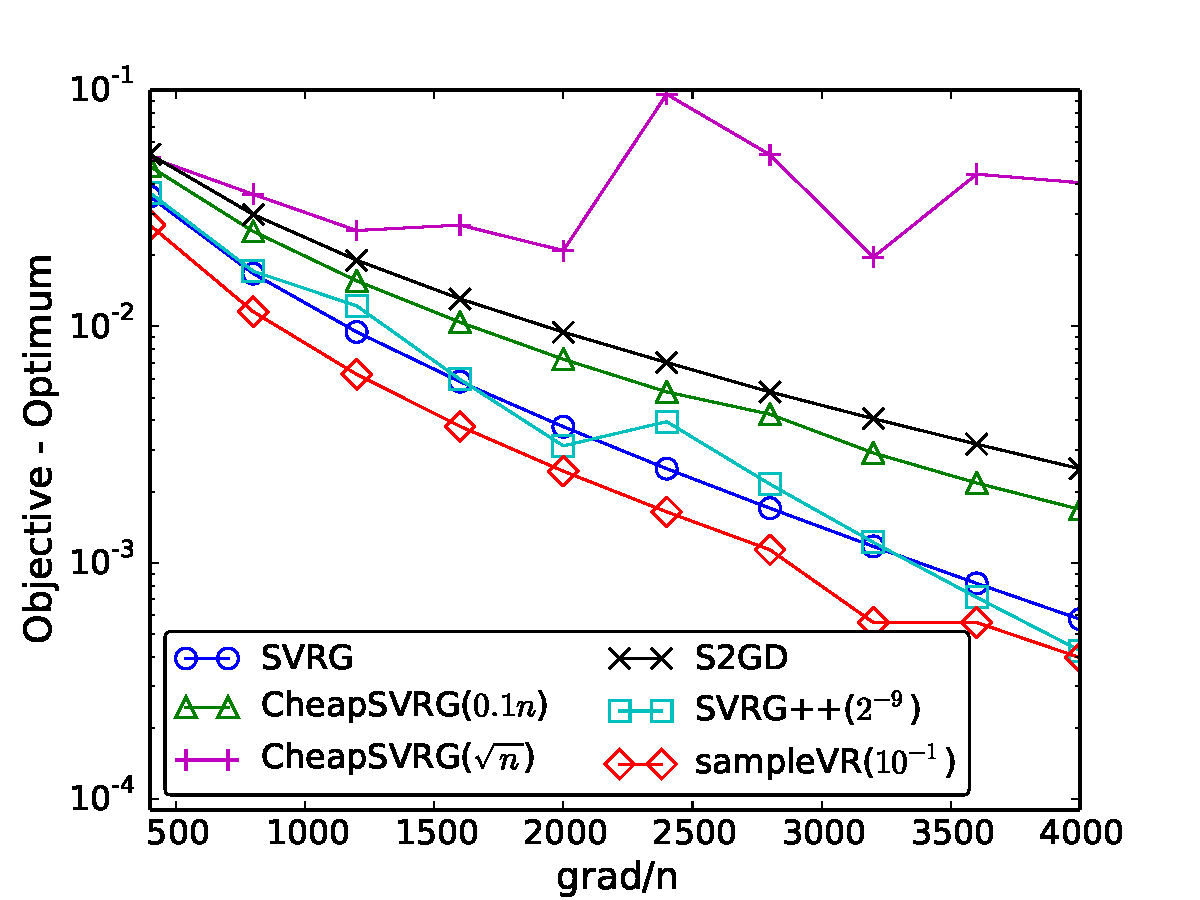
\includegraphics[width=0.5\columnwidth]{figure_ijcnn_convergence}\label{figure_ijcnn_convergence}}
\subfigure[colon-cancer]{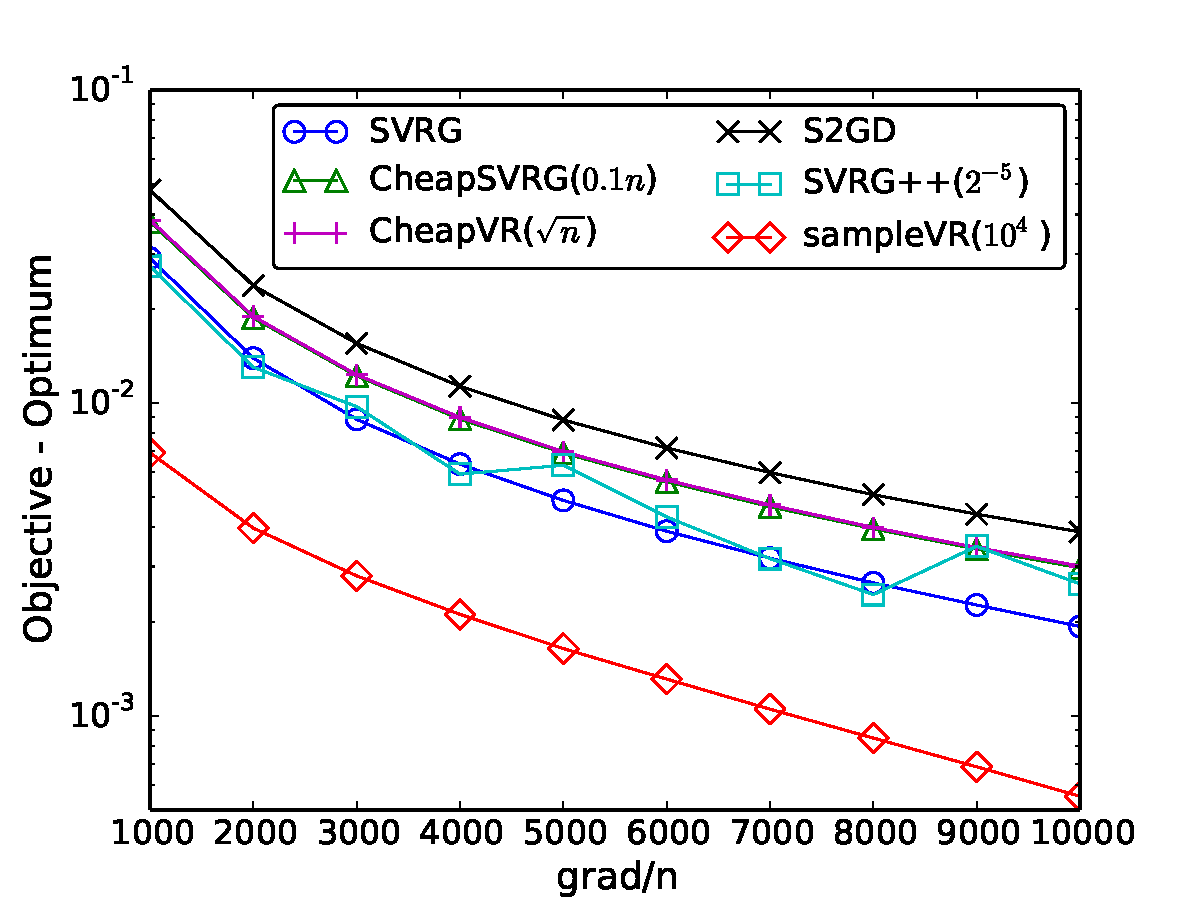
\includegraphics[width=0.5\columnwidth]{figure_colon-cancer_convergence}\label{figure_colon-cancer_convergence}}
\subfigure[duke-breast-cancer]{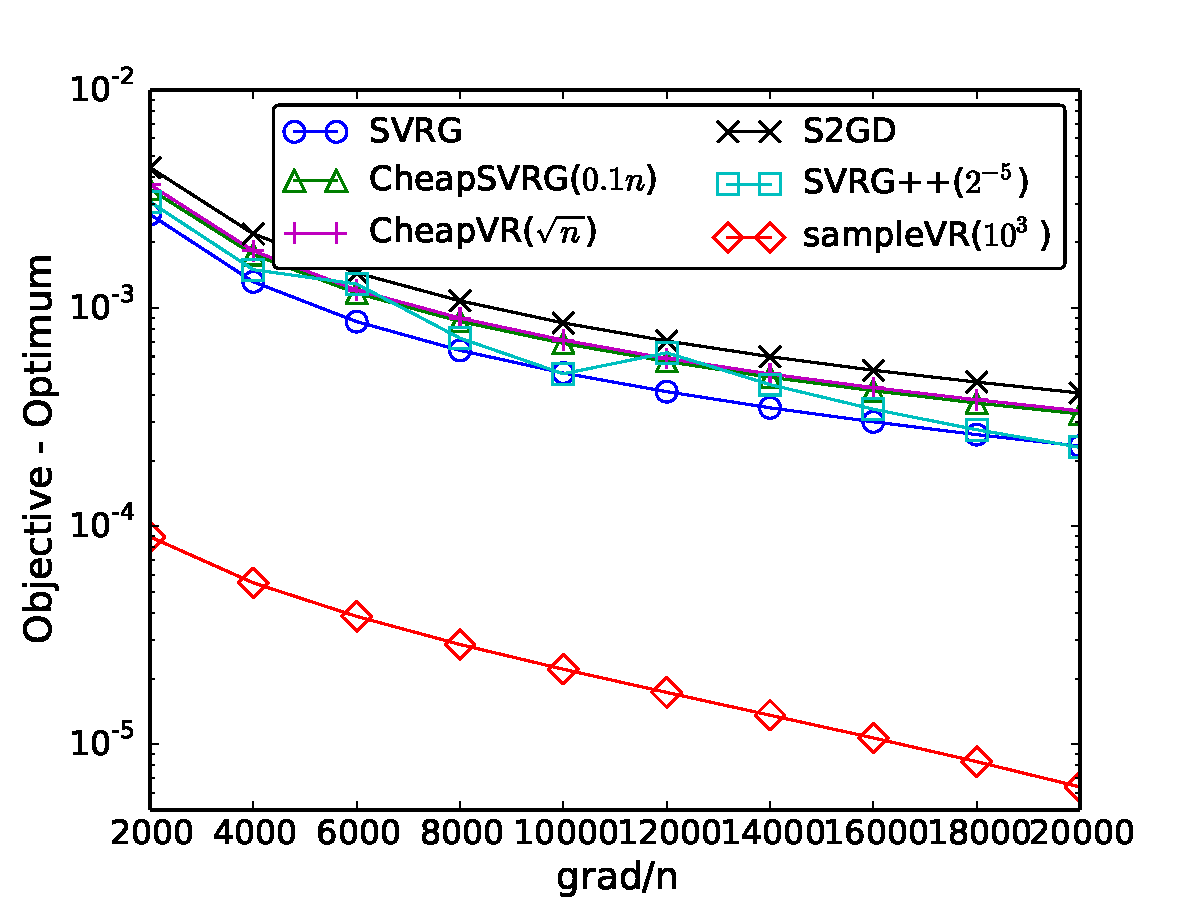
\includegraphics[width=0.5\columnwidth]{figure_duke_convergence}\label{figure_duke_convergence}}
\subfigure[a9a]{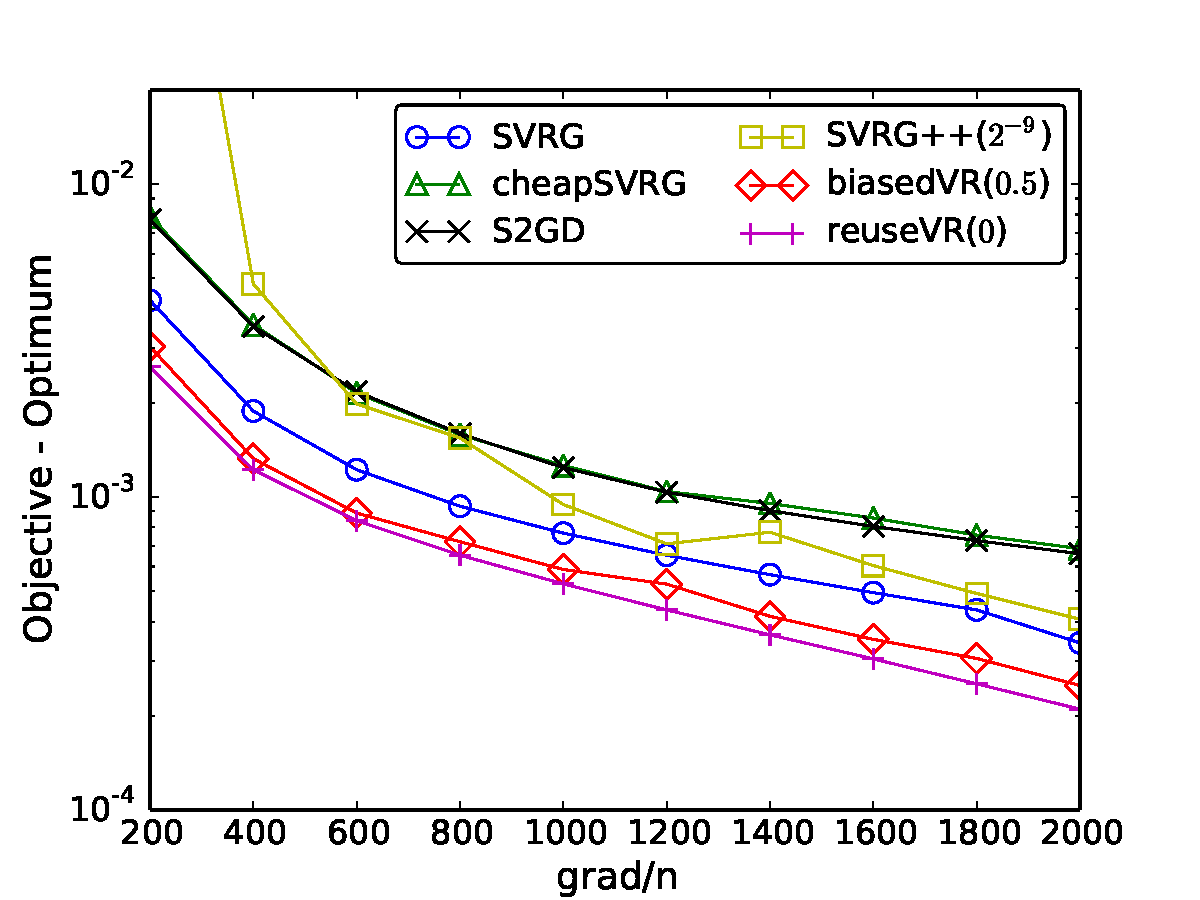
\includegraphics[width=0.5\columnwidth]{figure_a9a_convergence}\label{figure_a9a_convergence}}
\caption{\textsc{sampleVR} makes the training loss of the $l2$-regularised logistic regression tasks converge faster than the other existing algorithms.}
\label{figure_logistic_regression_convergence}
\end{figure*}

\begin{figure*}[t]
\centering
\subfigure[ijcnn1]{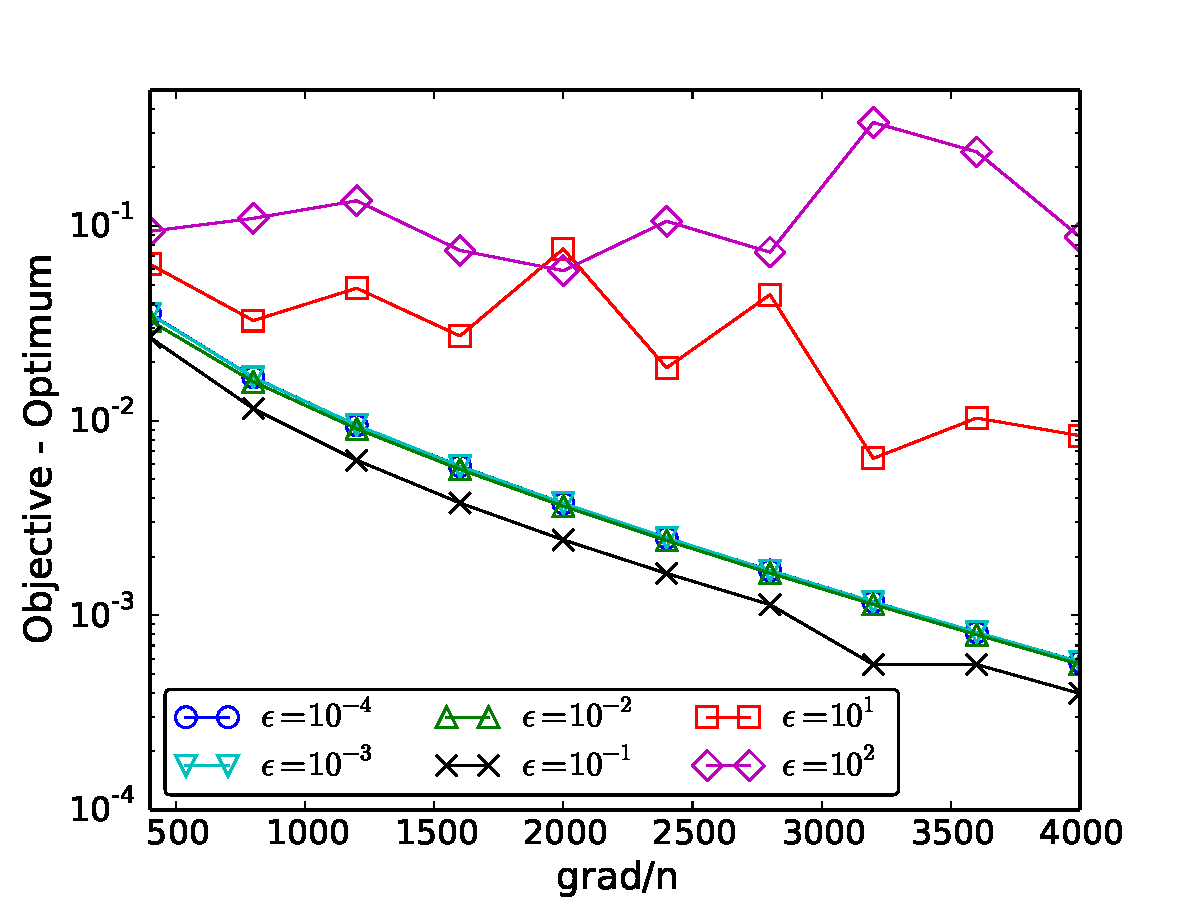
\includegraphics[width=0.5\columnwidth]{figure_ijcnn_rho}\label{figure_ijcnn_rho}}
\subfigure[colon-cancer]{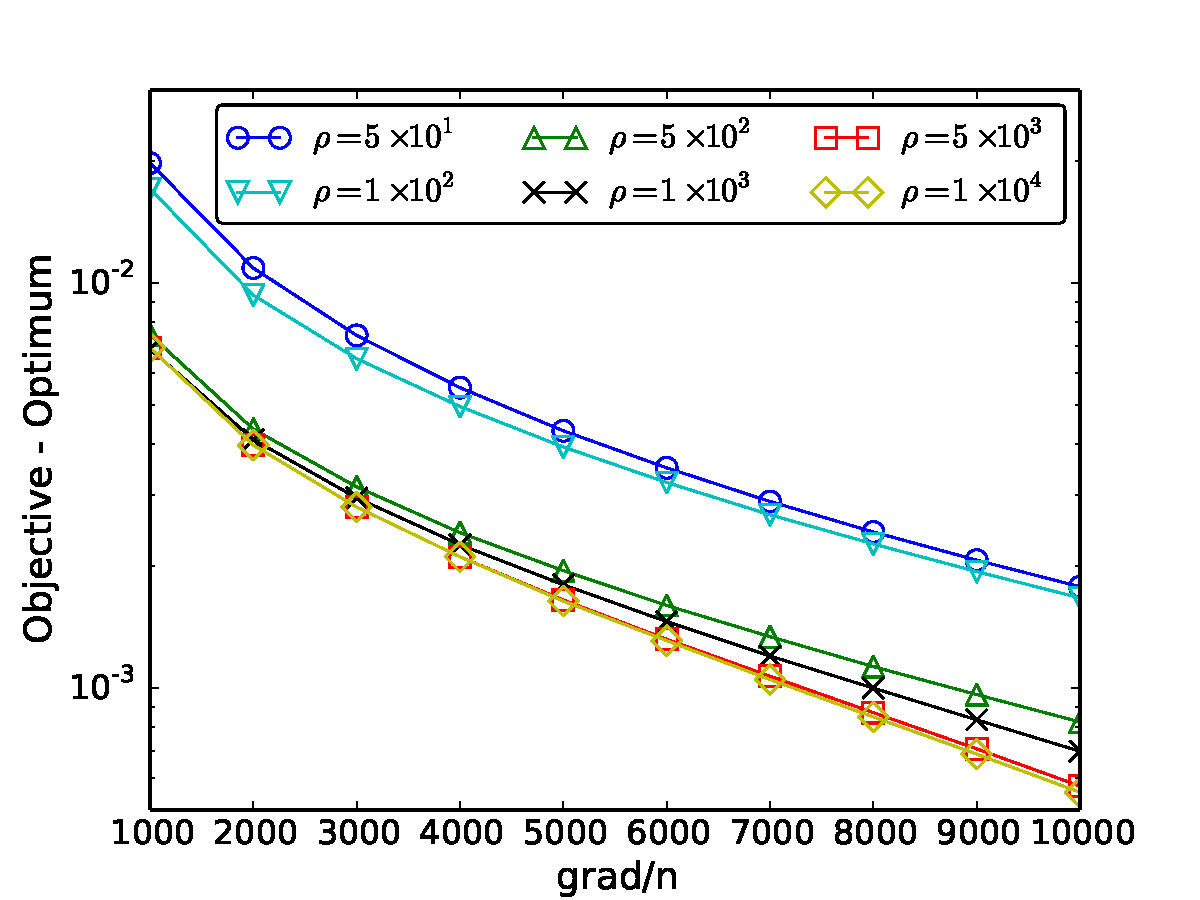
\includegraphics[width=0.5\columnwidth]{figure_colon-cancer_rho}\label{figure_colon-cancer_rho}}
\subfigure[duke-breast-cancer]{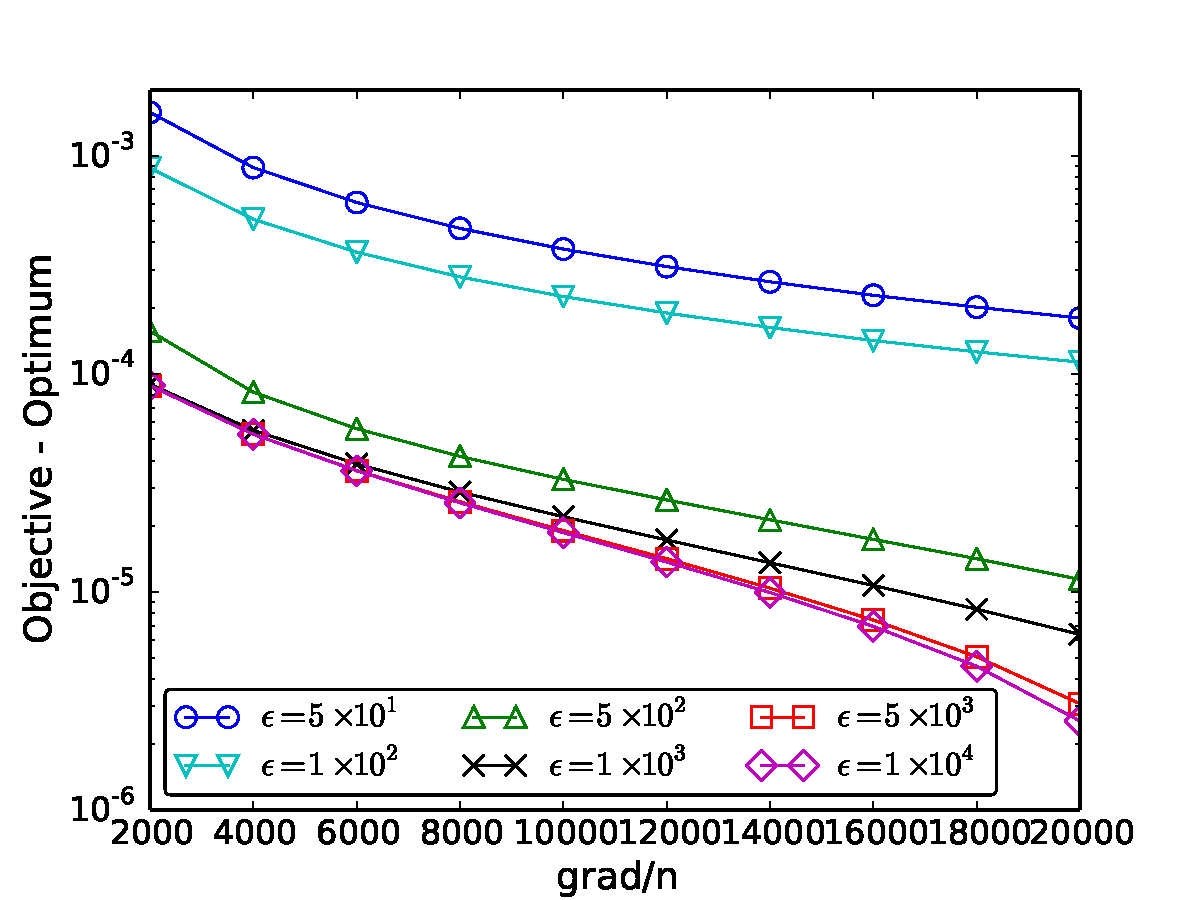
\includegraphics[width=0.5\columnwidth]{figure_duke_rho}\label{figure_duke_rho}}
\subfigure[a9a]{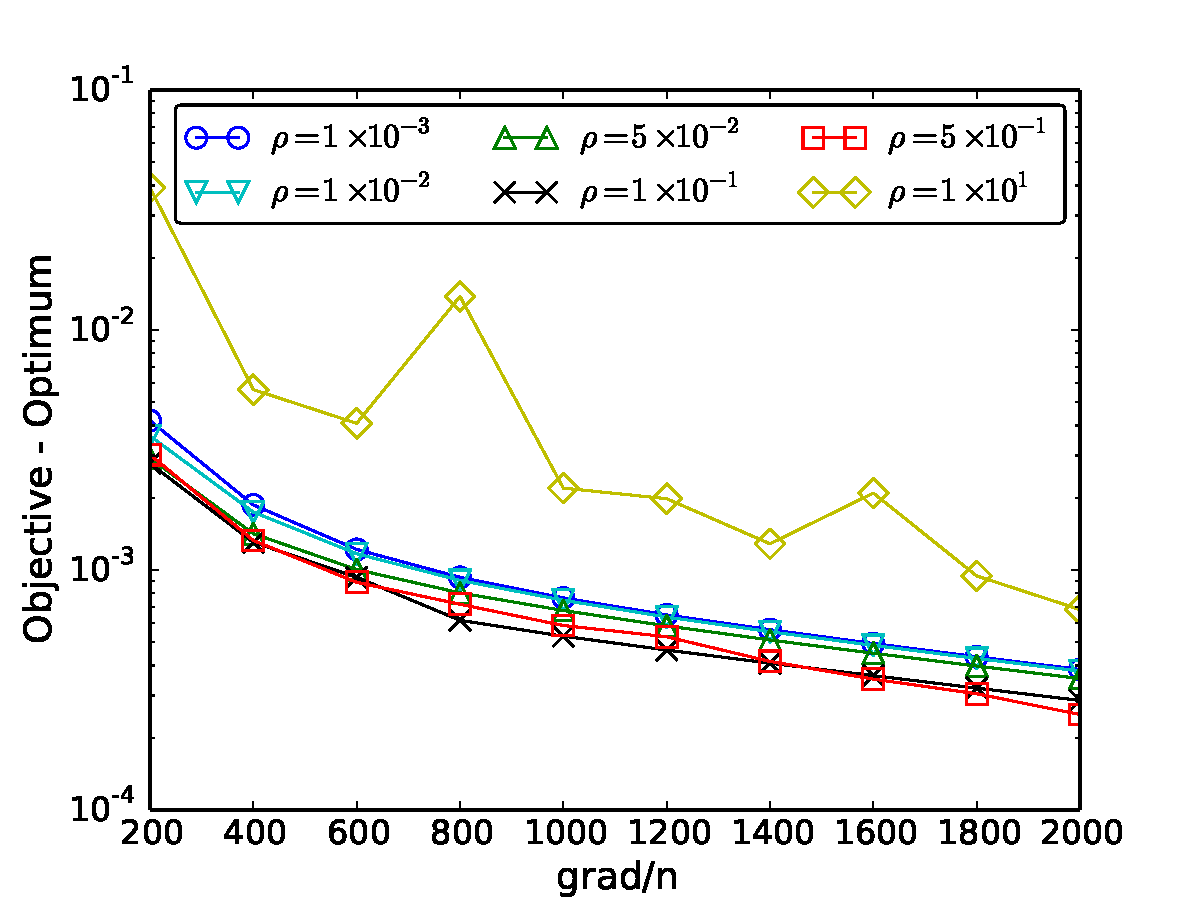
\includegraphics[width=0.5\columnwidth]{figure_a9a_rho}\label{figure_a9a_rho}}
\caption{Generally, \textsc{sampleVR} with a large $\epsilon$ has a better performance for the the $l2$-regularised logistic regression tasks. However,  the increase of the variance caused by an extremely large $\epsilon$ makes the convergence of the training loss slow down.}
\label{figure_logistic_regression_rho}
\end{figure*}



 As illustrated in Theorem \ref{Theorem_converge}, \textsc{sampleVR} makes the optimisation objective converge at a linear rate. To be honest,  the convergence performance is  not the best when comparing with SVRG  because that the ratio of the learning rate of \textsc{sampleVR} against that of \textsc{SVRG} is
\begin{equation}
\begin{array}{ll}
\frac{\delta^{\mathrm{\textsc{sampleVR}}}}{\delta^{\mathrm{SVRG}}} \mathrm{=} \frac{1+4L \mu m\eta^2}{\mu m \eta(1-2\eta L)} \mathrm{\times} \frac{1}{\frac{1}{\mu \eta(1-2L\eta)m} + \frac{2L\eta}{1-2L\eta}}  \\
\mathrm{=} \frac{1+4L\mu m \eta^2}{1+2L\mu m \eta^2} <2.
 \end{array} 
\end{equation} However, \textsc{sampleVR} has a significant advantage on the gradient complexity according to Theorem \ref{theorem_gradient_complexity}. For example, when the optimisation objective is strongly convex, and achieves $\mathbb{E}[F(\tilde{\omega}_s)\mathrm{-}F(\omega_\ast)] \mathrm{\le} \zeta$ with $\zeta\mathrm{=}\frac{1}{n}$, the gradient complexity of SVRG and its variants is $O\left(n \ln n\right)$ \citep{Allen2015UniVR}. But, the gradient complexity of \textsc{sampleVR}  is $O( \ln^2 n ) $. \textsc{sampleVR} thus  outperforms SVRG and its variants on the gradient complexity due to $\ln n \mathrm{\ll} n$.



 Although the estimation of the full gradient, i.e. $\dot{g}$ is unbiased, the variance between $\dot{g}$ and $g$ impedes convergence of the training loss, especially when the parameters get close to the optimum. This problem is mitigated in \textsc{sampleVR} by increasing the number of the sampled instances  over epochs linearly.     In specific, according to Assumption \ref{assumption_liptchiz}, every stochastic gradient $\nabla f_i(\omega)$ with $i\in\{1,2, ..., n\}$ is bounded by $L$, that is, $\parallel  \nabla f_i(\omega)  \parallel \le L$.  $\mathbb{E}\left(\frac{1}{k}\sum\limits_{i=1}^k\parallel  \nabla f_i(\tilde{\omega}_{s+1})  \parallel\right) \mathrm{=} \frac{1}{n}\sum\limits_{i=1}^n\parallel \nabla f_i(\tilde{\omega}_{s+1})\parallel$. Suppose $\chi  \mathrm{=} \frac{1}{k}\sum\limits_{i=1}^k\parallel \nabla f_i(\tilde{\omega}_{s+1})  \parallel - \frac{1}{n}\sum\limits_{i=1}^n\parallel \nabla f_i(\tilde{\omega}_{s+1})\parallel$, we obtain $P( | \chi | \ge \rho)  \mathrm{\le} 2e^{\frac{-2k\rho^2}{L^2}}$, according to Hoeffding's inequality. Let $\alpha \mathrm{=} P(| \chi | \ge \rho) \le 2e^{\frac{-2k\rho^2}{L^2}}$. Such the probability represents the level of significance, i.e. $\alpha$   for a confidence interval  around the expectation of size $2\rho$. Let $\epsilon = \frac{2\rho^2}{L^2}$. If we require at least $k$ instances  to acquire $(1\mathrm{-}\alpha)$-confidence interval $[-\rho, \rho]$,  $k$ should satisfy
\begin{equation}
\label{equ_estimate_samples_lower_bound}
k\ge - L^2\frac{\log \frac{\alpha}{2}}{2\rho^2} = - \frac{\log \frac{\alpha}{2}}{2\rho^2/L^2} = - \frac{\log \frac{\alpha}{2}}{\epsilon}.
\end{equation}  Therefore, $k$ is increased with the decrease of $\epsilon$, and thus the variance caused by the estimation  is reduced.  However, $k$ is not trivial to be identified. On one hand, a large $k$ leads to much computation cost to obtain the estimation of the full gradient.   On the other hand, a small $k$ causes much variance between  the full gradient and its estimation.  $\textsc{sampleVR}$ increases $k$ linearly, which achieves a good tradeoff between the time efficiency and the variance. The theoretical and empirical studies have shown that $\textsc{sampleVR}$ decreases much gradient complexity and  thus outperforms its counterparts.


\section{Performance evaluation}
\label{sect_performance_evaluation}


\begin{figure*}[t]
\centering
\subfigure[mg]{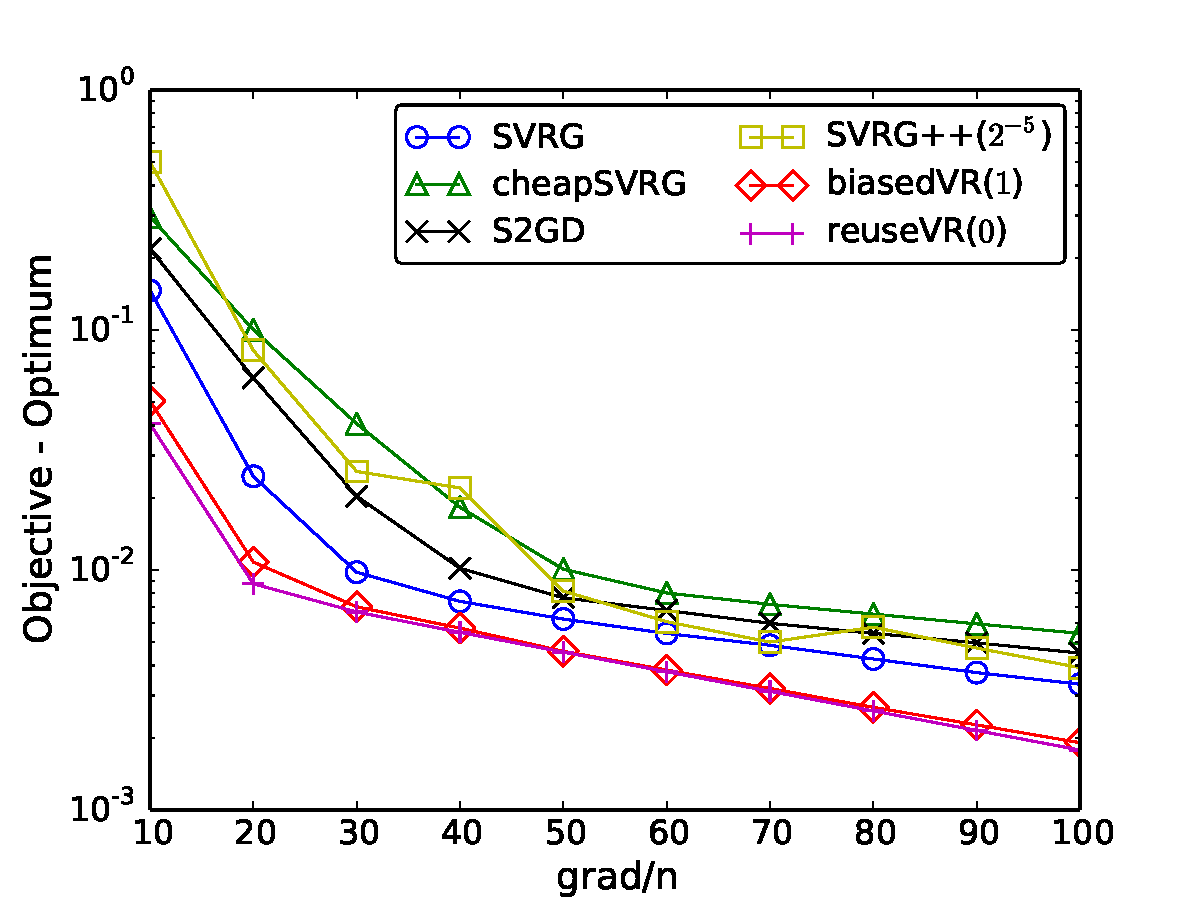
\includegraphics[width=0.5\columnwidth]{figure_mg_convergence}\label{figure_mg_convergence}}
\subfigure[cpusmall]{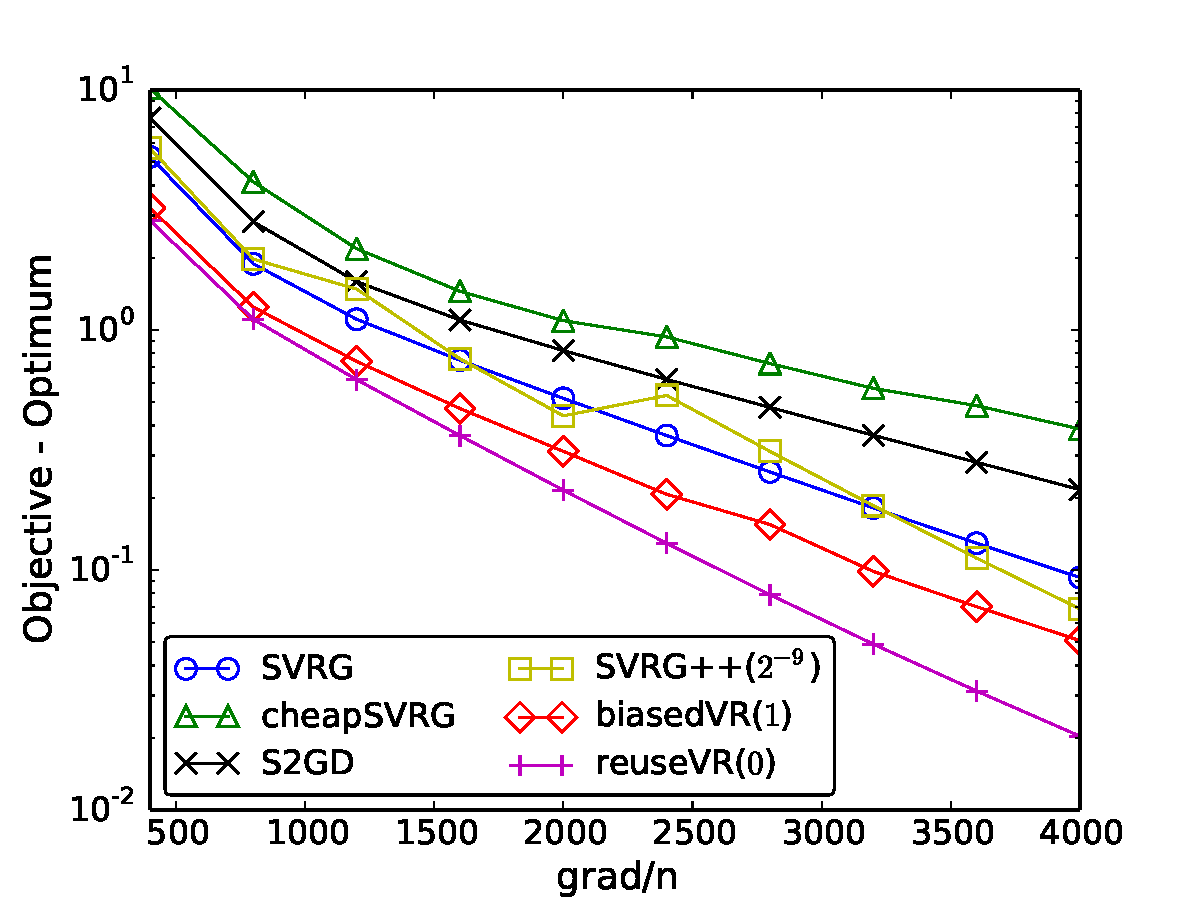
\includegraphics[width=0.5\columnwidth]{figure_cpusmall_convergence}\label{figure_cpusmall_convergence}}
\subfigure[yearPredictionMSD]{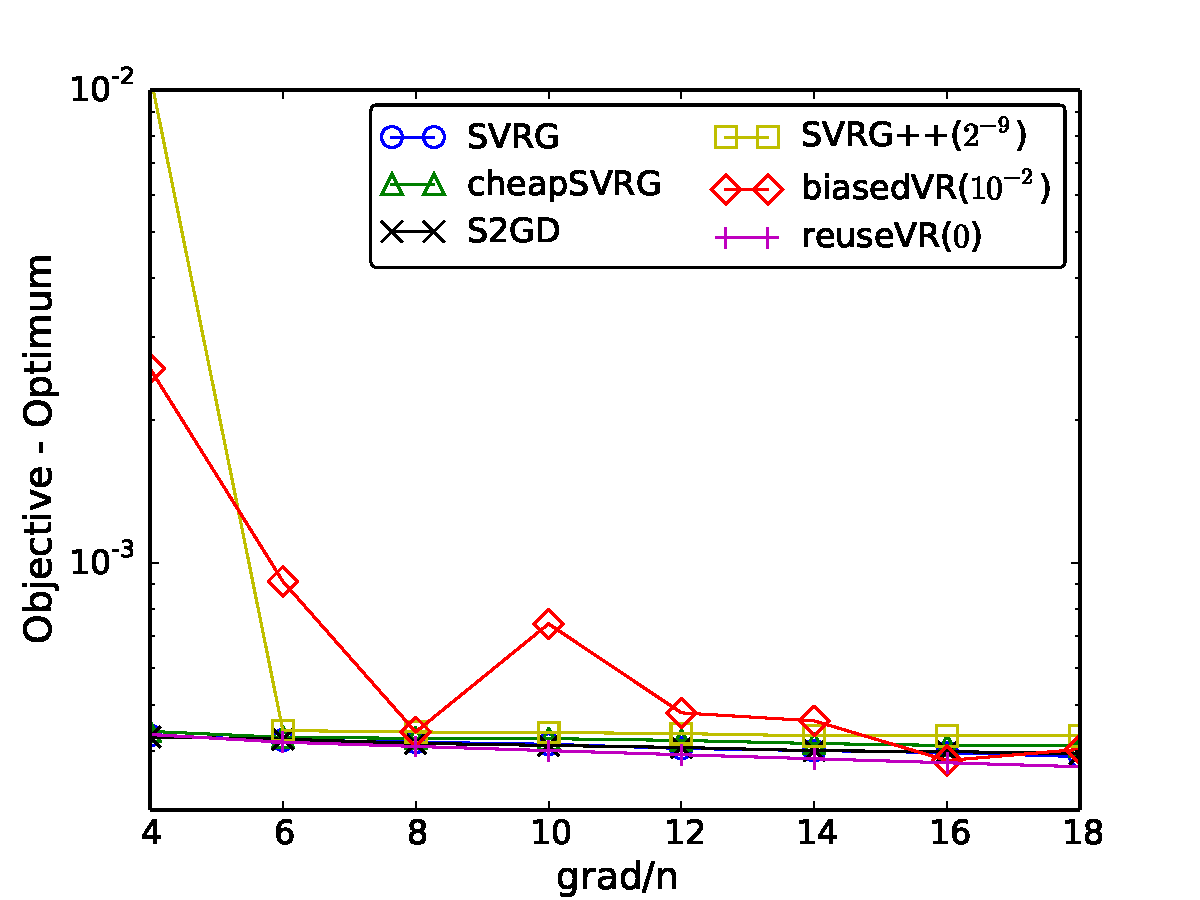
\includegraphics[width=0.5\columnwidth]{figure_year_convergence}\label{figure_year_convergence}}
\subfigure[space-ga]{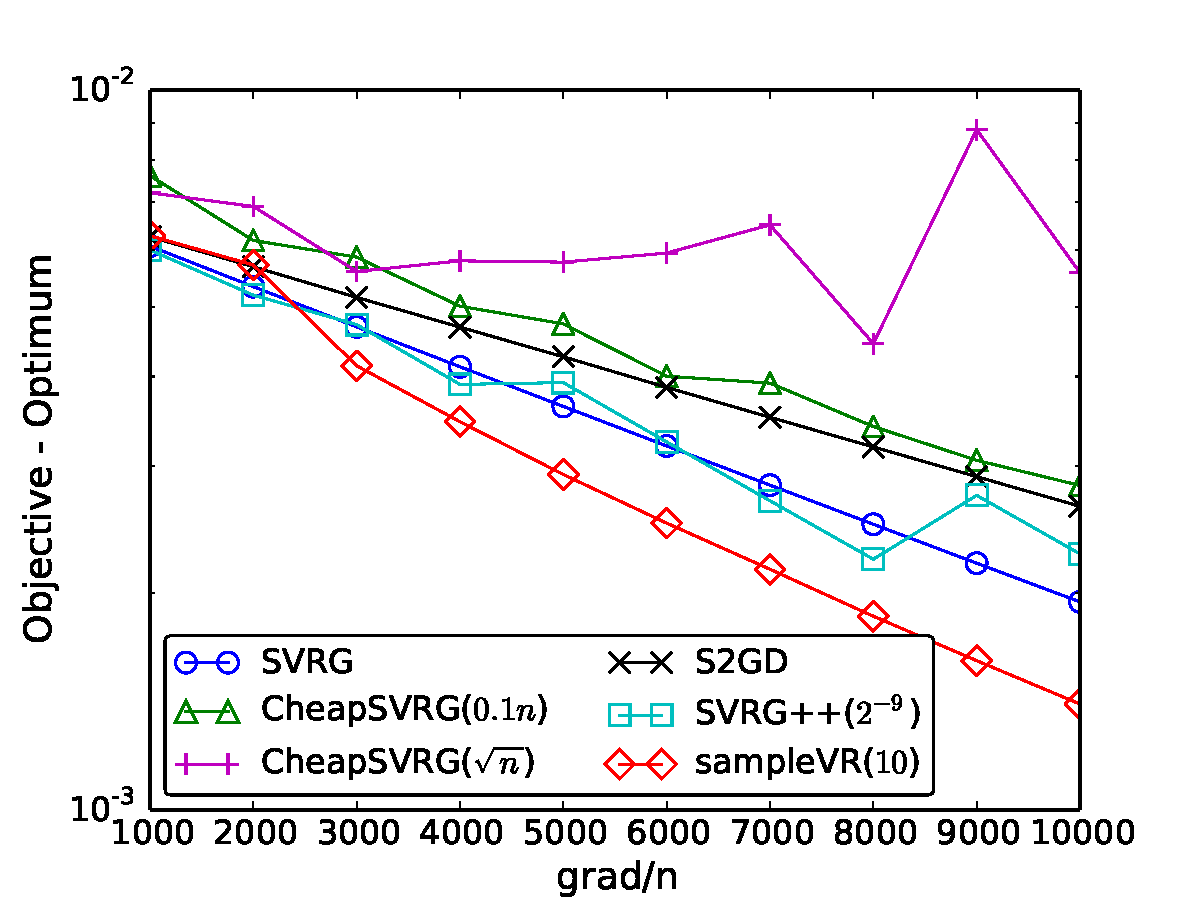
\includegraphics[width=0.5\columnwidth]{figure_space-ga_convergence}\label{figure_space-ga_convergence}}
\caption{Generally, \textsc{sampleVR}  outperforms the other existing algorithms on the convergence of the training loss when conducting the ridge regression tasks.}
\label{figure_ridge_regression_convergence}
\end{figure*}



\begin{figure*}[t]
\centering
\subfigure[mg]{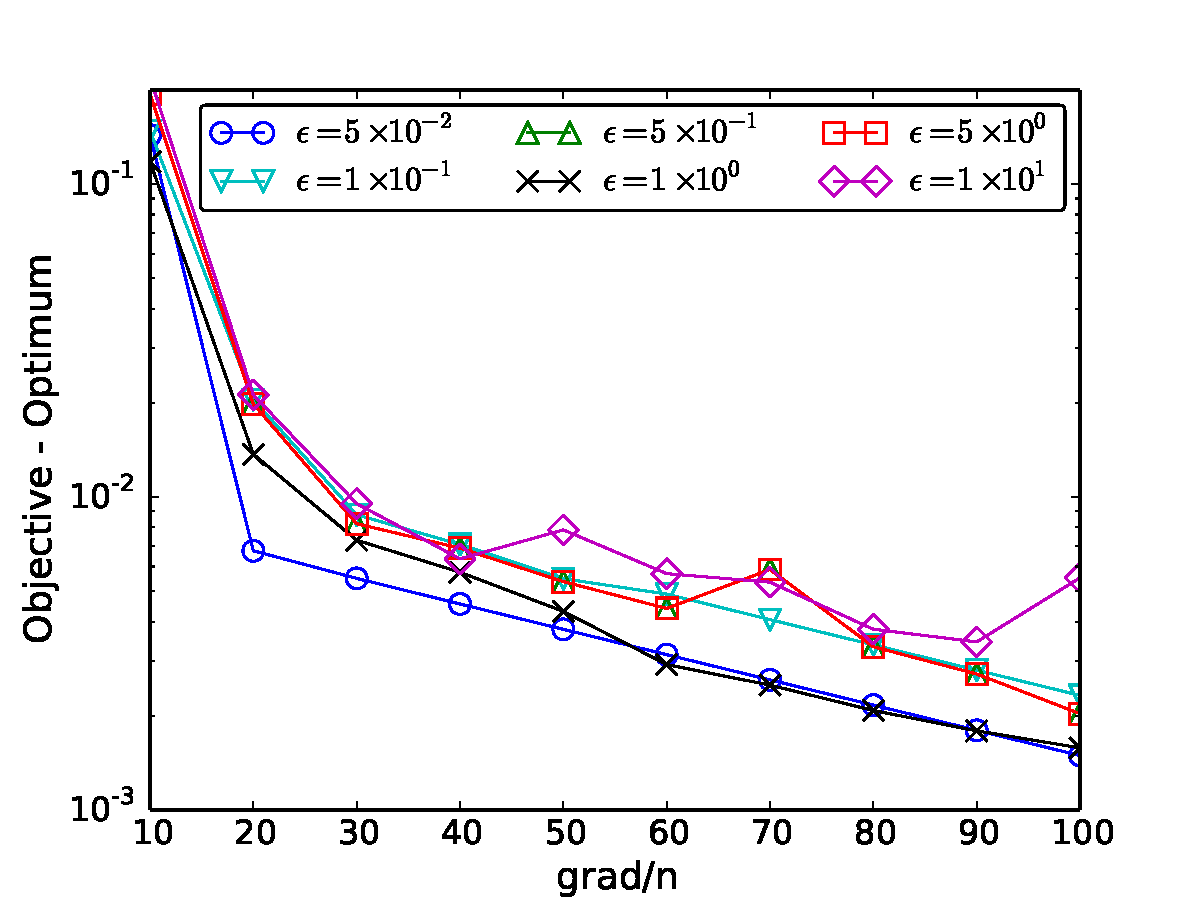
\includegraphics[width=0.5\columnwidth]{figure_mg_rho}\label{figure_mg_rho}}
\subfigure[cpusmall]{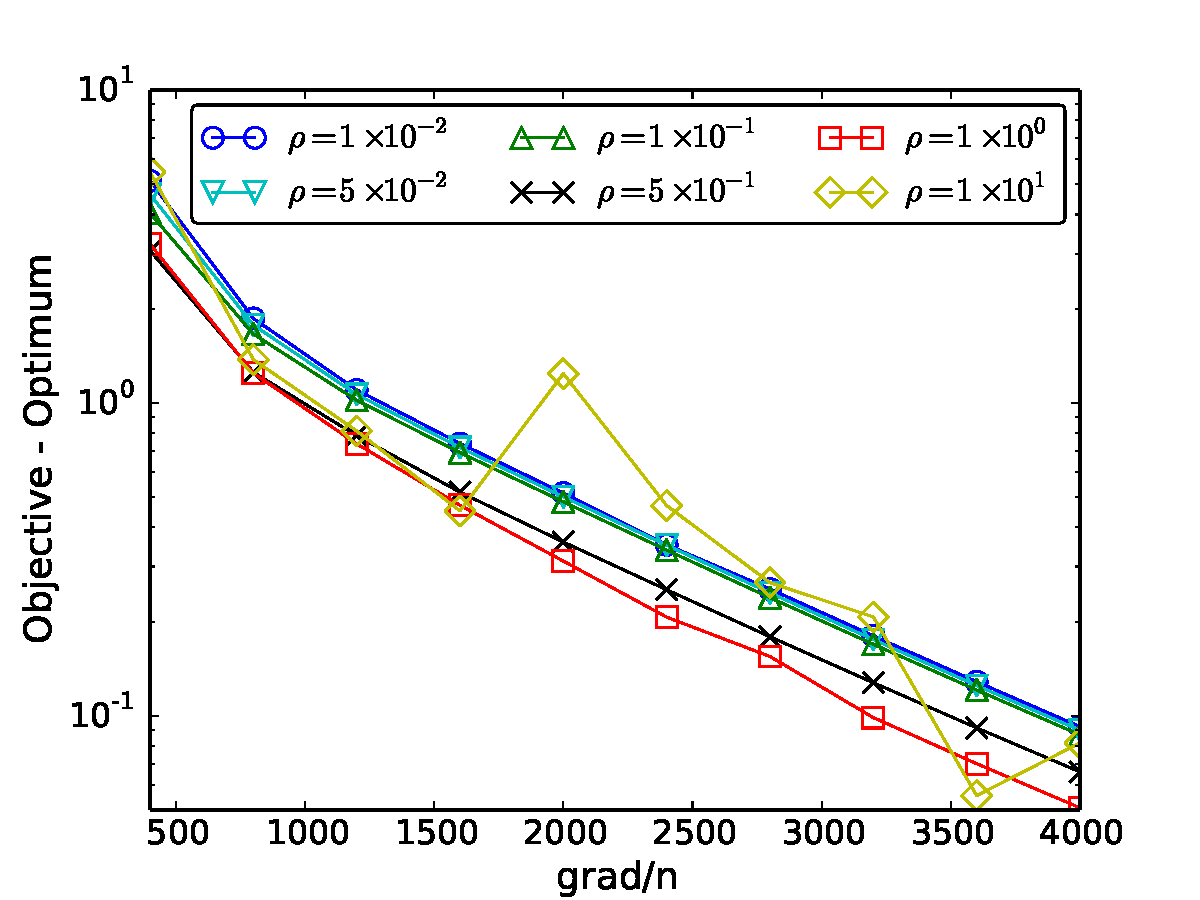
\includegraphics[width=0.5\columnwidth]{figure_cpusmall_rho}\label{figure_cpusmall_rho}}
\subfigure[yearPredictionMSD]{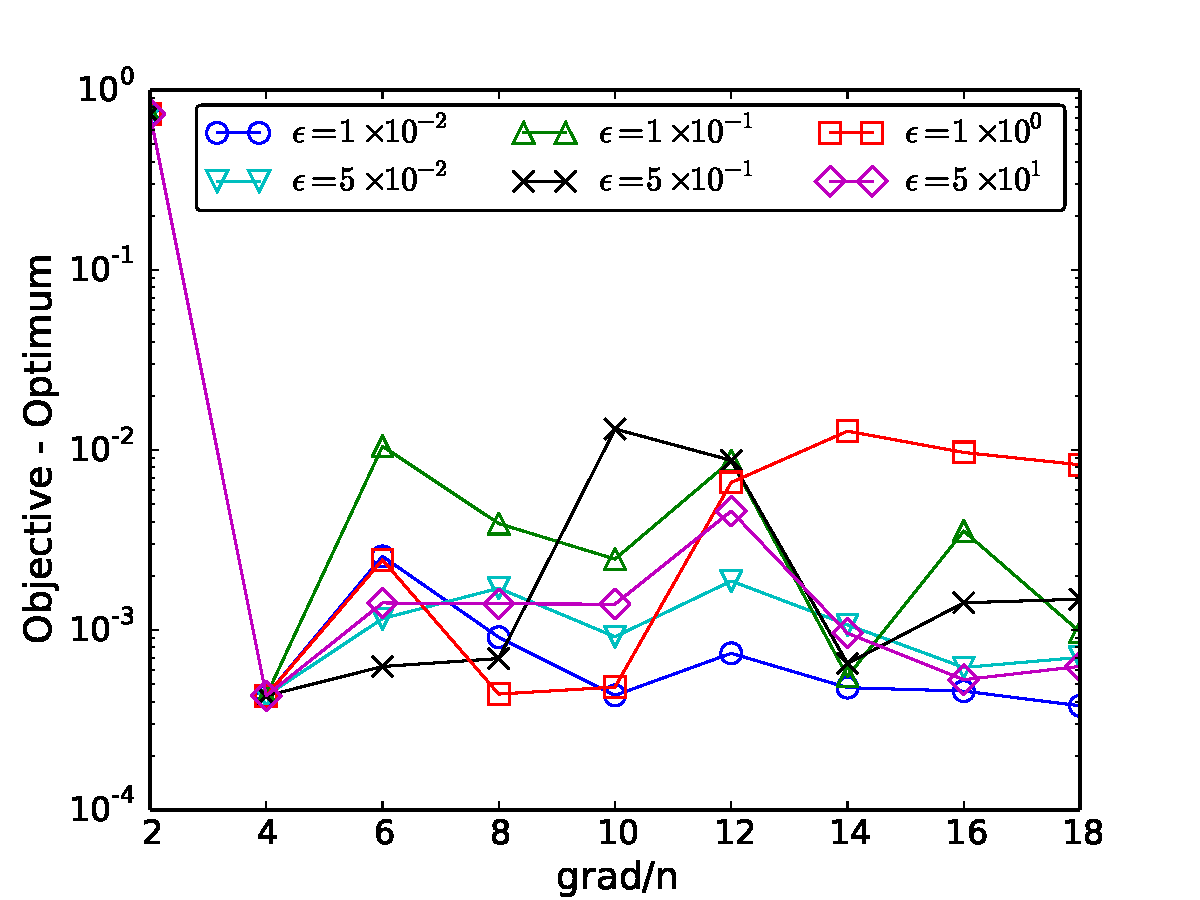
\includegraphics[width=0.5\columnwidth]{figure_year_rho}\label{figure_year_rho}}
\subfigure[space-ga]{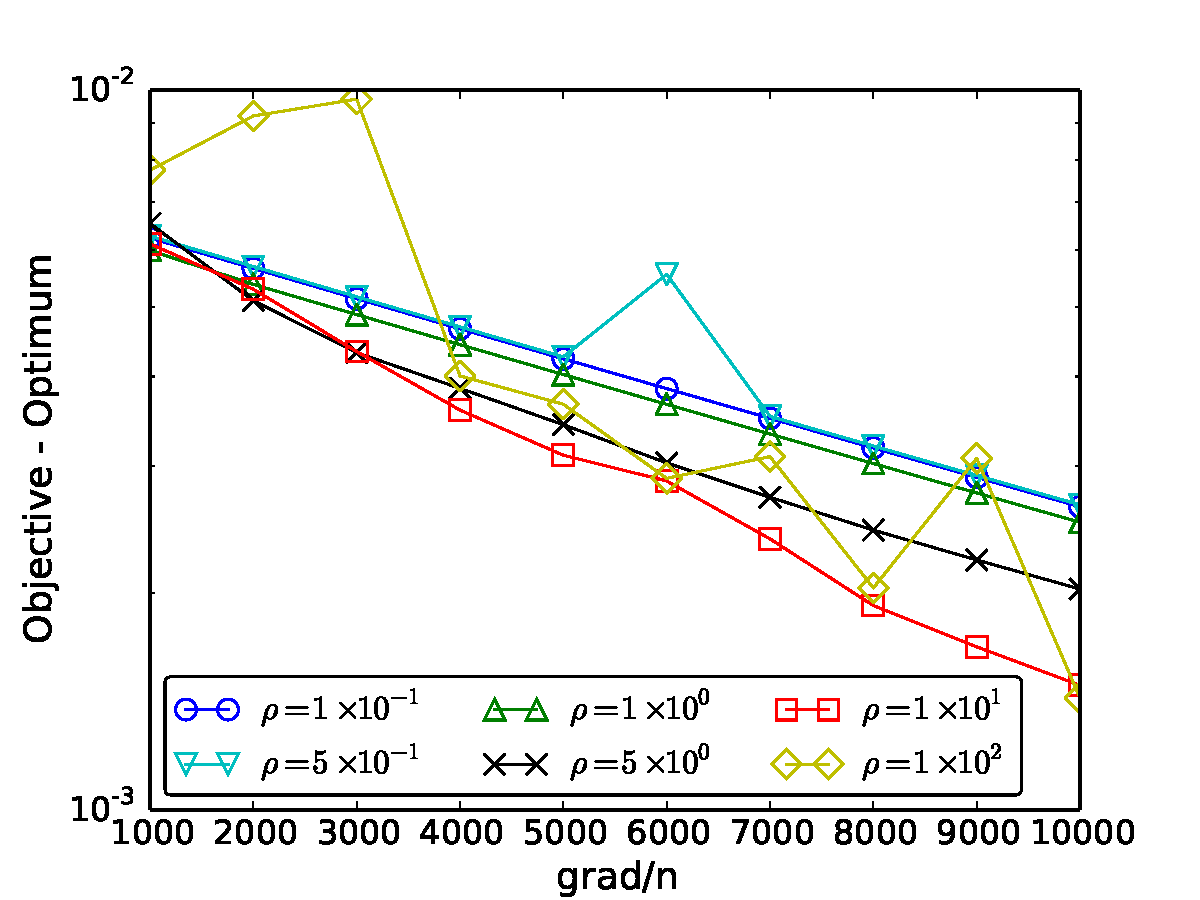
\includegraphics[width=0.5\columnwidth]{figure_space-ga_rho}\label{figure_space-ga_rho}}
\caption{A large $\epsilon$ leads to the fast convergence of the training loss for \textsc{sampleVR} when conducting the ridge regression tasks. However, the performance of  \textsc{sampleVR} is impaired  due to the increase of variance when $\epsilon$ is set to be too large.}
\label{figure_ridge_regression_rho}
\end{figure*}



\subsection{Experimental settings}
\label{sect_experimental_settings}
The existing variants of SGD with the variance reduction technique, including SVRG, S2GD, SVRG++, \textsc{CheapSVRG} have been used to conduct the performance evaluations with our proposed algorithm, i.e. \textsc{sampleVR}. The number of sampled instances in \textsc{CheapSVRG} is identified as $0.1n$ and $\sqrt{n}$ where $n$ represents the size of the training data.
Those algorithms are evaluated on eight datasets, including ijcnn1, colon-cancer, duke-breast-cancer, a9a, mg, cpusmall, yearPredictionMSD, and space-ga. All of those datasets are public on the LibSVM website. \footnote{http://www.csie.ntu.edu.tw/$\sim$cjlin/libsvmtools/datasets/} 

First, those algorithms are compared by conducting the $l2$-regularised logistic regression tasks on the datasets: ijcnn1, colon-cancer, duke-breast-cancer, and a9a. When the label of an instance is set to be $1$ or $-1$, the loss function of the $l2$-regularised logistic regression tasks is:
$$
\min\limits_\omega \frac{1}{n}\sum\limits_{i=1}^n \log(1+e^{-y_i \omega^\mathrm{T} x_i }) + \lambda \parallel \omega \parallel^2.
$$ Second, we compare those algorithms by conducting ridge regression tasks on the other four datasets, i.e. mg, cpusmall, yearPredictionMSD, and space-ga. The loss function of the ridge regression tasks is:
$$
\min\limits_\omega \frac{1}{n}\sum\limits_{i=1}^n\left(\omega^{\mathrm{T}}x_i-y_i\right)^2 + \lambda \parallel \omega \parallel^2.
$$ We set $\alpha$ to be $0.01$, $\lambda$ to be $10^{-5}$, and the learning rate, i.e. $\eta$ to be $10^{-4}$ for all evaluations.  The epoch size $m_s$ in SVRG and \textsc{CheapSVRG} is set to be the size of training data, i.e. $m_s\mathrm{=}n$. The maximal epoch size in S2GD is set to be the size of training data, i.e. $n$.    The x-axis in all  figures represents the computational cost. The computational cost is measured by the number of gradient computations divided by  the size of training data, i.e. $n$. The y-axis in all the figures denotes training loss residual which is the training loss minus the optimum. Here, the optimum is estimated by running the gradient descent for a long time. The value in the bracket of the legend of SVRG++ and \textsc{sampleVR} represents the initial epoch size divided by the size of the training data, i.e. $n$ and $\epsilon$ according to Algorithm \ref{algorithm_sampleVR}, respectively.

\subsection{$l2$-regularised logistic regression}
\label{sect_performance_evaluation_convergence}
As illustrated in Figure \ref{figure_logistic_regression_convergence}, we compare the performance of all the algorithms by conducting $l2$-regularised logistic regression tasks.  It is obvious that our proposed algorithm, i.e. \textsc{sampleVR} makes the training loss converge linearly, and outperforms other existing algorithms.   The main reason is that  \textsc{sampleVR} replaces   the full gradient with an estimation, thus getting rid of the time-consuming calculations of the gradient.  Although the estimation of the full gradient is used in  \textsc{CheapSVRG}, the number of sampled instances in \textsc{CheapSVRG}  is set before the running of the algorithm and then keep a constant such as $\sqrt{n}$. The constant number of sampled instances leads to much computation cost at first and much variance in the end during the training of the parameters.    Instead,  \textsc{sampleVR} increases the number of sampled instances linearly, and thus achieves a good tradeoff between time efficiency and variance. 
Additionally, the comparison of the  performance of \textsc{sampleVR} by varying   $\epsilon$ is shown  in Figure \ref{figure_logistic_regression_rho}. \textsc{sampleVR} generally obtains a better performance with a large $\epsilon$. It is because that the number of the sampled instances becomes small with a large $\epsilon$ according to Equation \ref{equ_estimate_samples_lower_bound}, which  reduces the computational cost significantly. However, as illustrated in Figure \ref{figure_ijcnn_rho} and \ref{figure_a9a_rho}, if $\epsilon$ is set to be too large, the number of the sampled instances becomes extremely small.  Thus, the large variance makes the training loss converge slowly. 


\subsection{Ridge regression}
\label{sect_performance_evaluation_convergence}
As illustrated in Figure \ref{figure_ridge_regression_convergence}, we report the comparison of the performance by using all the algorithms to  conduct  ridge regression tasks. \textsc{sampleVR} has a better performance for the datasets mg, cpusmall, and space-ga than the existing algorithms significantly. The main reason is that \textsc{sampleVR} uses an unbiased estimation of the full gradient, instead of costing much time to compute it.  Although \textsc{sampleVR} does not outperform other algorithms for the dataset yearPredictionMSD at the beginning of the train process, its performance is comparable to the other algorithms, and finally shows the advantage over most of the existing algorithms.  As illustrated in Figure \ref{figure_ridge_regression_rho}, the performance of \textsc{sampleVR} has been compared by varying $\epsilon$. It is significant that the variance becomes noticeable with the increase of $\epsilon$. It is because that a large $\epsilon$ leads to few sampled instances  according to Equation \ref{equ_estimate_samples_lower_bound}, incurring much variance in the estimation of the full gradient. Moreover,  an extremely small  $\epsilon$  impairs  the performance of \textsc{sampleVR}. The reason is that such a small $\epsilon$ leads to a large number of the instances, thus incurring  much calculations of gradients.   It is noting that the best setting of $\epsilon$  in different datasets varies a lot, for example $10^{-2}$ in yearPredictionMSD and $10$ in space-ga. The best method to tune $\epsilon$ will be studied in the future work. Generally, a practical method  is to  tune the value of the $\epsilon$ on a subset of the training data to obtain the best setting.



\section{Conclusion}
\label{sect_conclusion}
This paper first analyses the  variance reduction technique   from a new prospective in a general framework, i.e. EUI. We report the results of the lower and upper bounds of the variance. Then, a new variant of SGD with the variance reduction technique, i.e. \textsc{sampleVR} is proposed. \textsc{sampleVR} replaces the full gradient by using its estimation, accelerates the convergence of training loss significantly. The theoretical and  extensive empirical studies show that  \textsc{sampleVR} outperforms its counterparts significantly.

\bibliography{reference}
\bibliographystyle{aaai}





\end{document}
